\section[Scintillation detectors (Mark I./Beni)]{Scintillation detectors \label{sec:scintillators}}
\subsection{Start counter \label{sec:st}}

The Start Counter (ST) detector, shown in Fig.~\ref{fig:st-overview-drawing}
surrounds the target
region and covers about 90\% of the solid angle for particles
originating from the center of the target. It is designed to operate
at tagged photon beam intensities of up to $10^8$ photons per second
in the coherent peak. It has a high degree of segmentation to limit
the the per-paddle rates. The time resolution is less than 350 ps
RMS. The Start Counter provides a timing signal that is releatively
independent of particle type and trajectory (because of its proximity
to the target), can provide particle identification via $dE/dx$, and
can be used in the Level 1 trigger.

\begin{figure}[!htb]
\centering
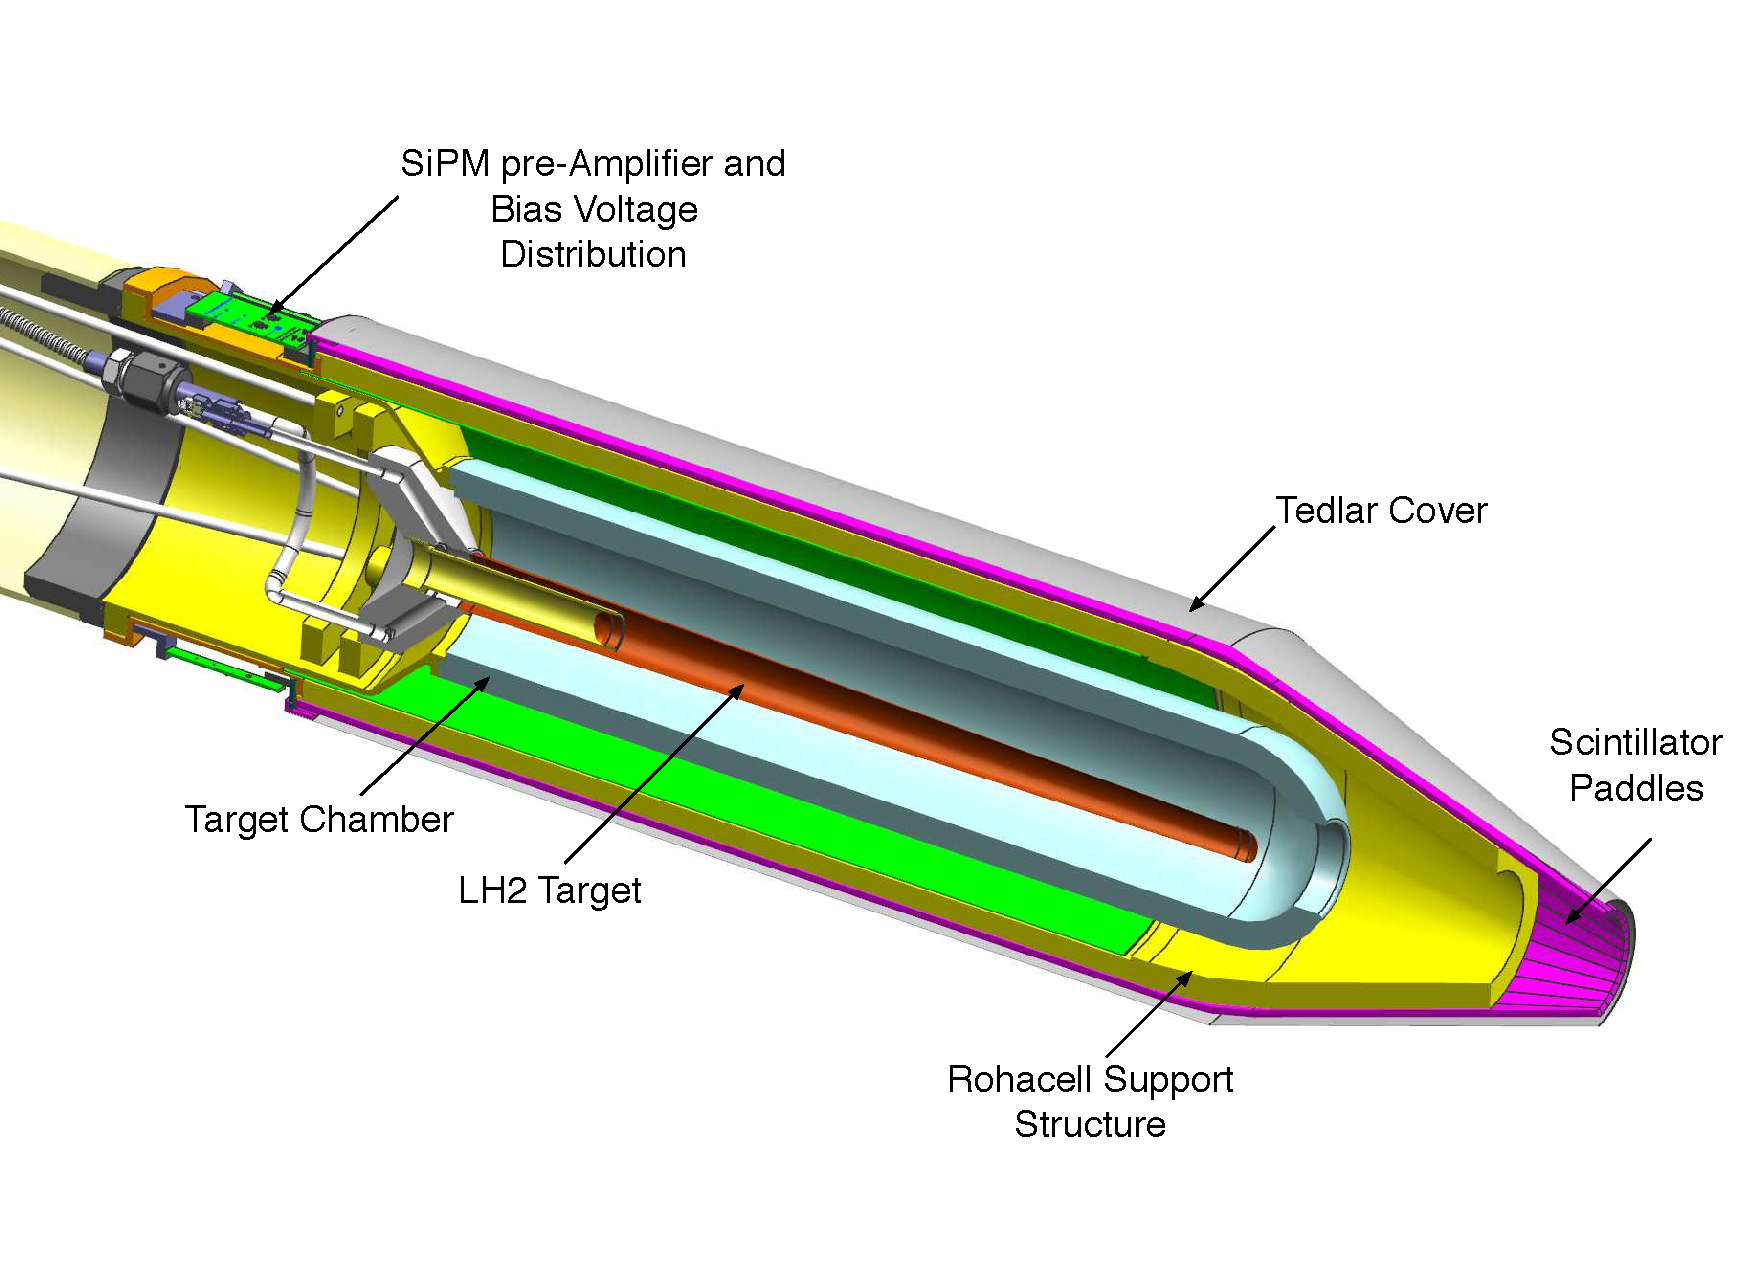
\includegraphics[width=1.0\columnwidth]{figures/start_counter_all.pdf}
\caption{The \gx{} Start Counter mounted to the liquid $\mathrm{H_2}$
  target assembly.  The beam goes from left to right down the central
  axis.\label{fig:st-overview-drawing}}
\end{figure}

\subsubsection{Detector Description}

The ST consist of 30 scintillator paddles arranged in a cylinder for most of
its length with a ``nose'' section that bends towards the beam line at
the downstream end. EJ-200 scintillator from Eljen
Technology\footnote{Eljen Technology, https://eljentechnology.com/products/plastic-scintillators.
	}
was selected. EJ-200 has a decay time
of 2.1~ns and an attenuation length of 380~cm. Silicon
photomultiplier (SiPM) detectors were use as light sensors [specs?]. These were
not affected by the 2 T[?] magnetic field produced by the GlueX
solenoid. The SiPMs were placed as close as possible to the upstream
end of each scintillator element to maximize light collection.

Each scintillator paddle started from stock 3~mm thick and 600 mm in
length. The paddles were bent at Eljen to create the nose section, and
then machined at McNeal Enterprises Inc.\cite{mcneal-reference} to
their final shape, including edges beveled at $6^\circ$ to minimize
loss of acceptance. The geometry for a single paddle is shown in
Fig.~\ref{figure:st-single-paddle-geometry}.

The scintillabor paddles are supported by a Rohacell closed-cell foam
structure. The Rohacell is 11 mm thick and is rigidly attached to an
aluminum support hub at its upstream end. The downstream support
extends partially into the nose section. The cylindrical length of the
Rohacell is further reinforced with three layers of carbon fiber, each
layer 650~$\mu$m thick. The assembly is made light-tigh with a Tedlar
wrapping. The Tedlar is attached to a plastic collar at the upstream
end. A summary of the materials used in the assembly are shown
schematically in Fig.~\ref{fig:st-materials}.

\begin{figure}[!htb]
  \centering
  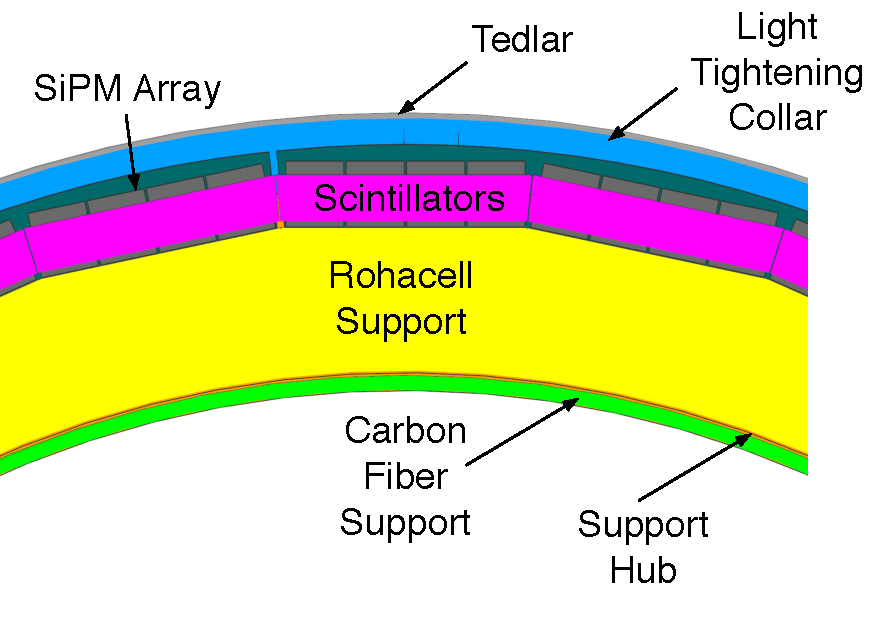
\includegraphics[width=1.0\columnwidth]{figures/st_materials.pdf}
  \caption{Start Counter materials.}
  \label{fig:st-materials}
\end{figure}

\subsubsection{Read-Out Electronics}

Each scintillator bar is read out with an array of four
magnetic-field-insensitive Hamamatsu S109031-050P multi-pixel photon
counters (MPPCs). Each MPPC consists of 3,600
$50 \times 50$ $\mu$m$^2$ avalanche photo-diode pixel counters
operating in Geiger mode. The signals from all pixels are summed. [no
  more mention of SiPM?] The scintillator is optically coupled to the
MPPCs through a 250 $\mu$m air gap. A schematic of the ST read-out electronics is shown in Fig.~\ref{fig:st-electronics}.

\begin{figure}[!htb]
  \centering
  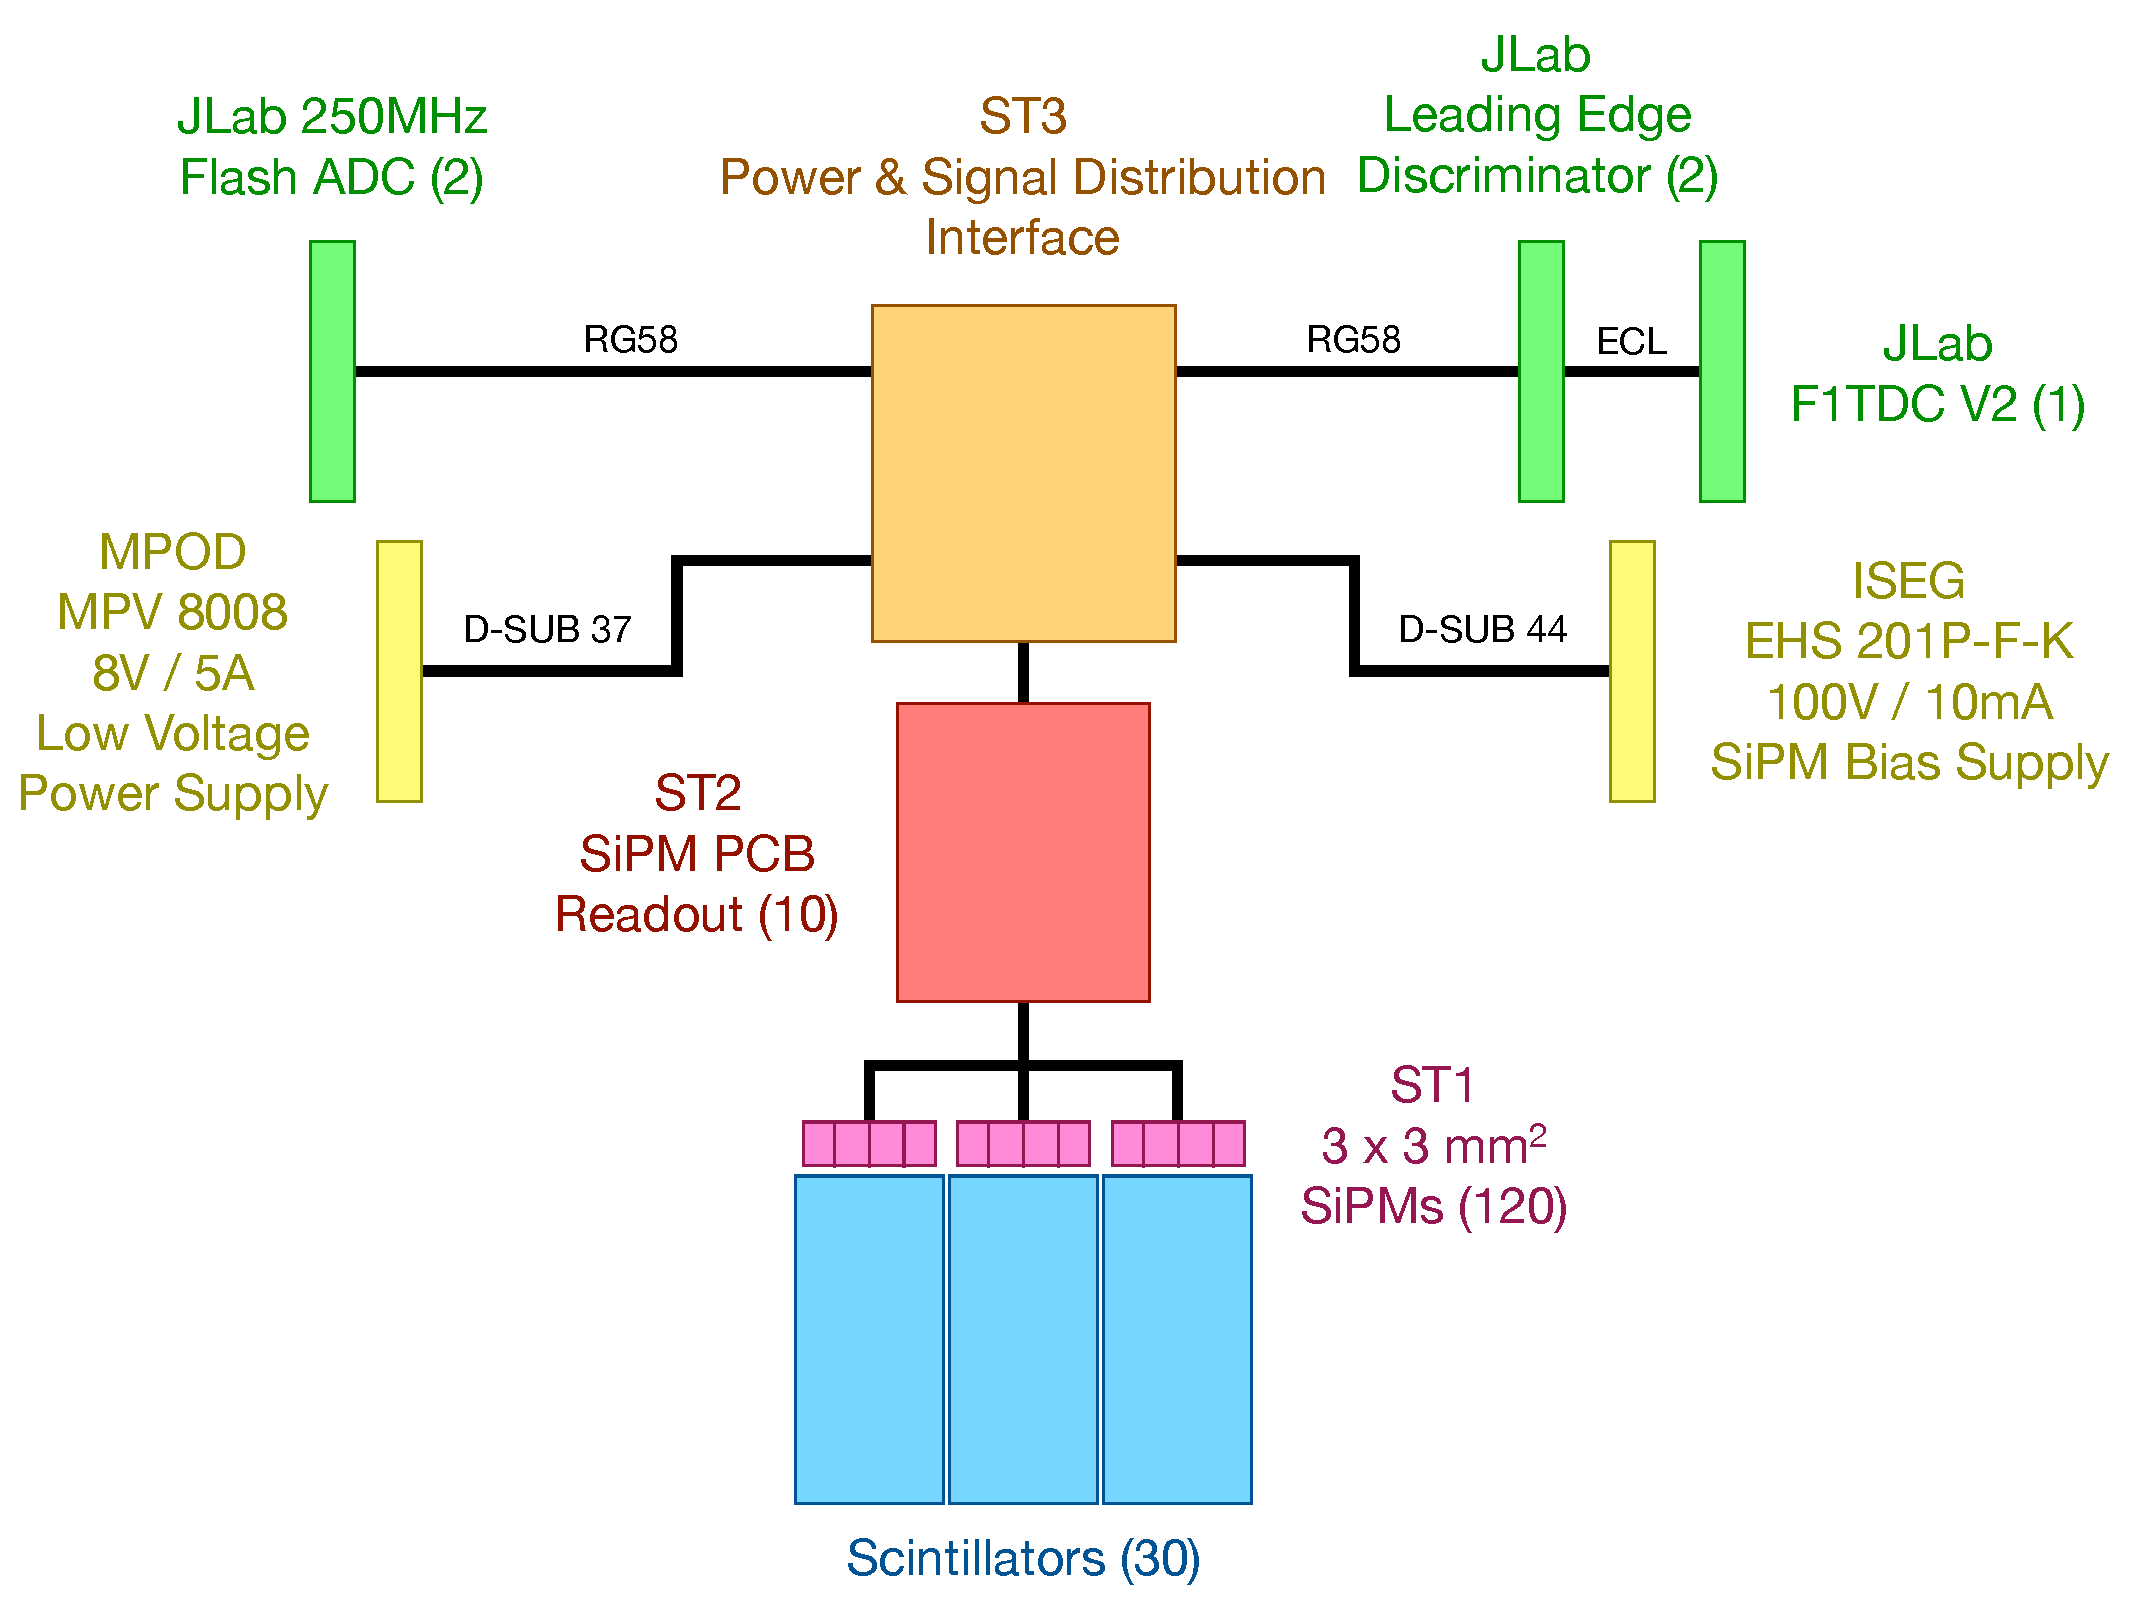
\includegraphics[width=1.0\columnwidth]{figures/st_electronics_diagram}
  \caption{Start Counter readout electronics diagram.  Numbers in 
    parenthesis indicate the total for the system.}
  \label{fig:st-electronics}
\end{figure}

The read-out electronics are deployed on three separate board designs,
``ST1,'' ``ST2,'' and ``ST3.'' The ST1 and ST2 boards are located
directly upstream of the end of the scintillator array, ST3 is located
further upstream, outside the bore of the solenoid magnet, adjacent to
the beam pipe.

The ST1 board houses the MPPCs themselves as well as a thermocouple for
temperature monitoring. Each ST1 board services three scintillator
paddles (twelve MPPCs per ST1 board). There are ten ST1 boards altogether. An ST1 board is shown in Fig.~\ref{fig:st-ST1}.

\begin{figure}[!htb]
  \centering
  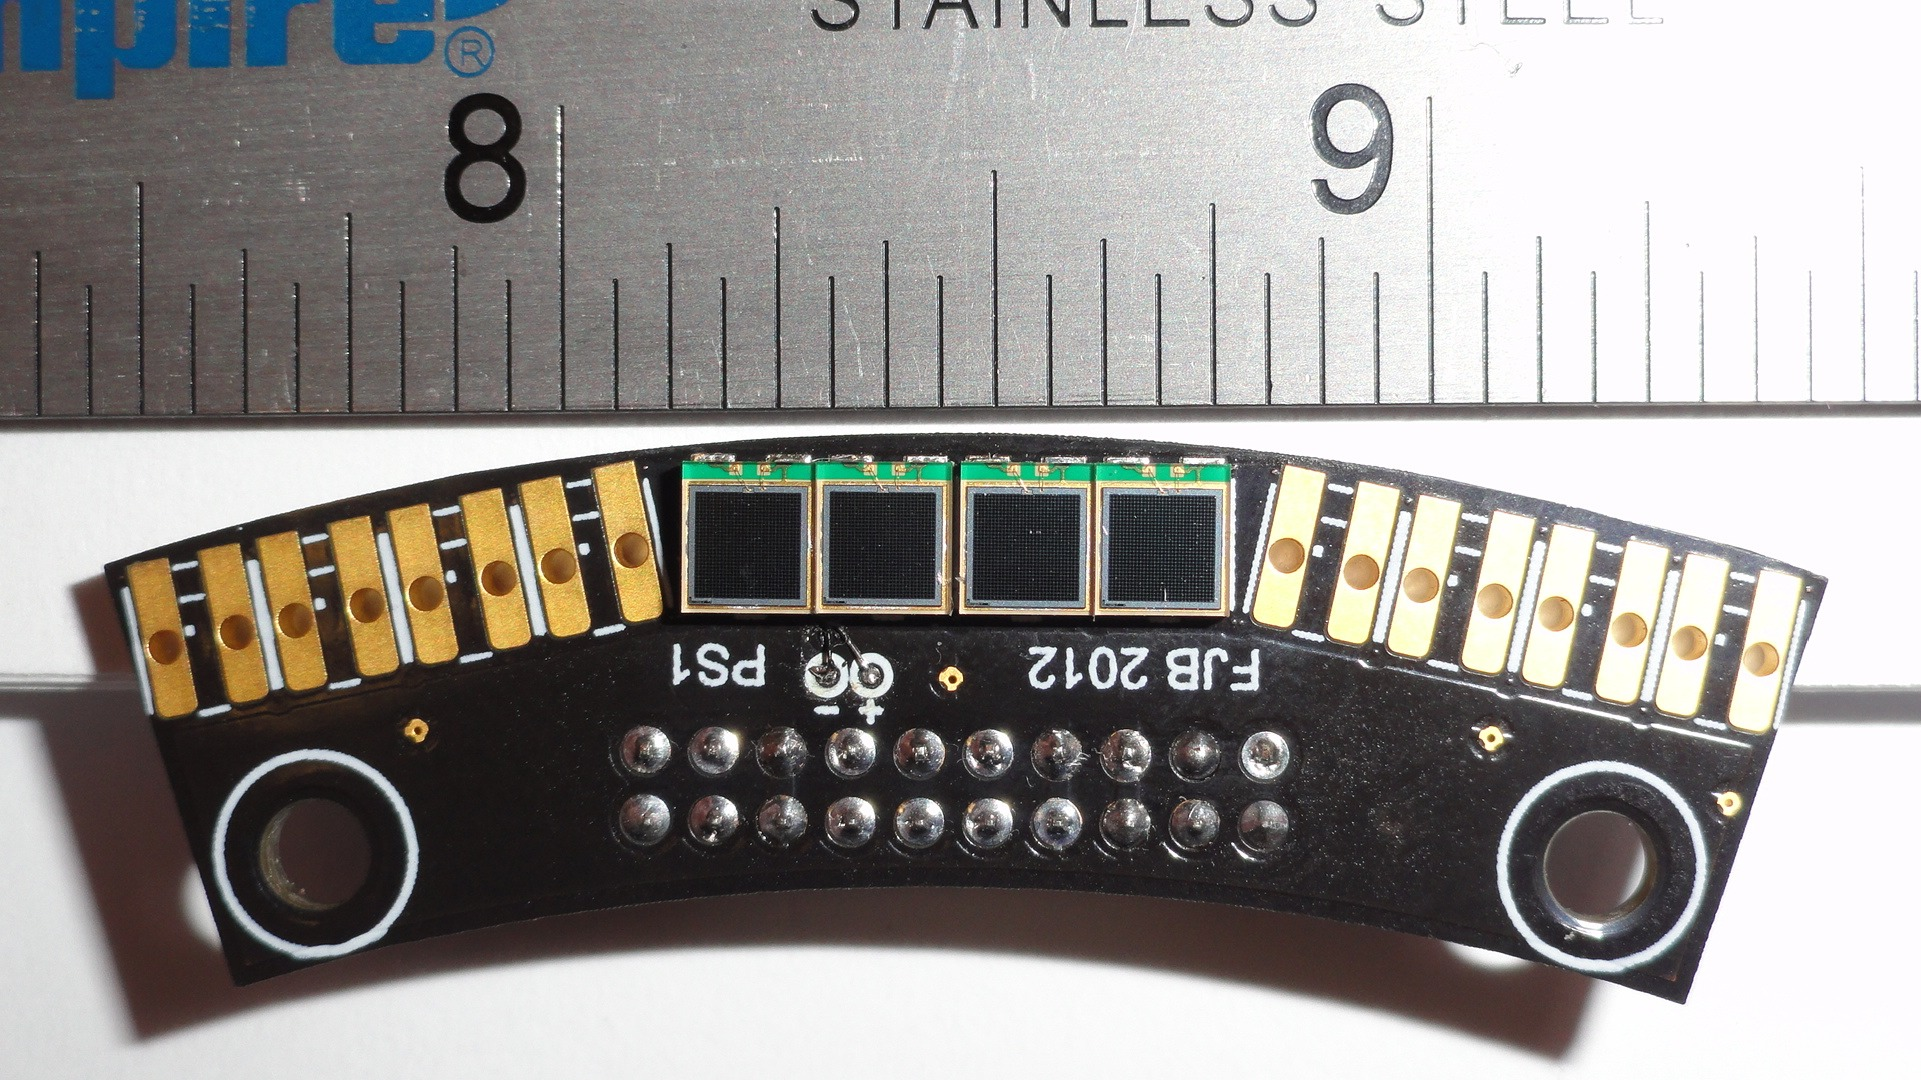
\includegraphics[width=1.0\columnwidth]{figures/st1_ruler}
  \caption{ST1 of Start Counter readout system.  Only the central array 
    is populated with SiPMs.  Approximately 72\% of the scintillator light 
    is collected at the upstream end.  The ST readout has 10 ST1 units in 
    total.  The ruler shown above is in inches.}
  \label{fig:st-ST1}
\end{figure}

For each ST1 board there is a corresponding ST2 board that services
all three electronic channels. For each channel there is a
pre-amplifier whose output is split. One side of the signal goes to a
buffer and then to a Flash ADC (FADC), the other goes to a
5$\times$~amplifier and is sent from there to a discriminator and TDC.

There is one ST3 provides an interface for distribution of low-voltage
power for the electronics and bias voltages for the MPPCs. It also
serves as a patch panel for the FADC, discriminator, and thermocouple
signal output cables.

\subsubsection{Calibration}

Calibrations are performed to correct measurements for the effects of
time-walk, light propagation time, and light attenuation

{\bf Time-Walk Correction}

Since the detector signal is sent to both a Flash ADC and a TDC, the time from the the FADC, which is largely independent of pulse amplitude, is used to measure the time walk seen by the TDC as a function of pulse amplitude as measured by the FADC. The resulting curve is fit to an empirical function to apply the correction and the procedure is done on a channel-by-channel basis.


\subsection[Time-of-flight counters (Beni)]{Time-of-flight counters \label{sec:tof}}
The Time-of-flight (TOF) detector is a wall of scintillators located about 5.5~m downstream from the target and covers 
an angular region from 0.6$^{\circ}$ to 13$^{\circ}$ in polar angle. The detector has two planes of
scintillator paddles stacked in the horizontal and vertical direction, respectively. Most paddles are 252~cm long and 2.54~cm
thick with a width of 6~cm. 
The scintillator material is EJ-200 from Eljen technology.
To accommodate the photon beam to pass through a central region of 12~cm by 12~cm is kept
free of any detector material giving rise to four short paddle detectors with a length of 120~cm around the beam hole
in each detector plane. These paddles also have a width of 6~cm with a thickness of 2.54~cm. In order to keep the
count rate of the paddles well below 2~MHz the two inner most full length paddles closest to the beam hole do have a reduced width of 3~cm.
Light guides from UV transmitting plastic provide the coupling space between the scintillator and the PMT and allow the 
magnetic shielding to protect the photo cathode by extending about 5~cm past the entrance window. All paddles are wrapped
with a layer of a highly reflective material DF2000MA from 3M followed by a layer of strong black Tedla film to
protect against external light sources. 
The main purpose of the detector is to provide fast timing for charged particles passing through the detector thereby providing information for particle identification and to the determine the event RF beam bunch of the photon that initiated the event.

\subsection{Electronics \label{sec:scelectronics}}
The full length scintillator paddles are read out on both ends using photo multiplier tubes (PMT) from Hamamatsu~\footnote{Hamamatsu Photonics "https://www.hamamatsu.com/us/en/index.html"}. These tubes of type H10534 have 10-stages and are complete assemblies with high voltage base, casing and $\mu$-metal shielding. Due to the significant stray field from the spectrometer solenoid magnet additional external
shielding based on soft iron is necessary to protect the PMTs from the magnetic field.
The high voltage (HV) to the PMTs is provided by CAEN HV modules of type A1535SN initially controlled by a CAEN SY1527 main frame
later upgraded to a SY4527.
The PMT output is connected to a splitter by a 50' long cables (WHAT TYPES?). The signal is split by
an passive splitter into two equal amplituded signals. One signals is directly connected to a flash ADC250~\cite{Dong:2007}
analog to digital converter (fADC) while the second signal passes first through a leading edge discriminator (LED) before connecting to 
a high resolution TDC VX1290A form CAEN~\footnote{CAEN "https://www.caen.it/"}. The digitizer electronics (fADC250 and TDC) are mounted
in VXS crates controlled by custom electronics as described in Section~\ref{sec:online}.
The threshold of the leading edge discriminator is controlled for each channel separately and has an intrinsic
dead time of about 25~ns.
The readout threshold for
the fADC250 is one single value for all channels on a single 16 channel board and is set to the same value for
all ADC modules in the TOF. The data from the fADC250 is provided by the FPGA algorithm and consists
of two words per channel with information about pedestal, signal amplitude, signal integral and timing.
The VX1290A TDC is a multi hit high resolution TDC with a buffer of 
up to 8 words per channel. The intrinsic dead time of a TDC channel is XX~ns. The timing resolution is about 25~ps per TDC count.
Since these TDCs provide the best time measurements in the GlueX detector the timing of the accelerator RF signal is also
digitized using this electronics.

\subsection{Calibration and monitoring \label{sec:sccalib}}
A detailed description of the TOF detector can be found in~\cite{GlueXTOFNIM}. Since the TOF detector consists of two
planes of narrow paddles oriented orthogonal to each other it is possible to calibrate the full detector independent
of any other external detector information. The overlap region of two full length paddles from the two planes define
a 6~cm by 6~cm area for most paddles with a few 3~cm by 3~cm areas close to the beam hole. The separation between
the two detector planes is minimal as they are mounted on top of each other and as such are only separated by their wrapping
material. While the time-difference TD between the two ends of a paddle is related to the hit position along the paddle
the mean-time MT is related to the flight time of a particle from the vertex to the paddle. Therefor the MT for two overlapping
paddles must be the same when they are hit by the same particle passing through both of them while the hit position in the horizontal (x) and vertical (y) dimensions are defined by TD of the two paddles. This relationship between paddles can be
explored to calibrate all paddles with respect to each other in a complete internally consistent way.

In a first step, however, all times have to be corrected for time-walk because of the use of LED discriminators which
introduces a time shift that depends on the signal amplitude. Because the signal amplitude together with its timing
in the fADC250 has been recorded as well this relation between time at threshold and signal amplitude can be parametrized and corrected for.

After all full length paddles with readout on both ends have been calibrated they can be used to as reference counters
the calibrate the remaining 8 paddles that do have only single-ended readout as they have to accommodate for the photon
beam to pass through the detector at zero degree. Again the fact that in any overlap region of two paddles from different
planes the flight time of the particle from the vertex to the detector is identical the MT of the full length paddle is used
as reference time for the time from the single ended paddle. This relation will result in a peaking distribution with the peak
location representing the timing offset of these single-ended readout paddles. Ensuring that the distribution of all offset
parameters together will have a distribution with a mean of zero will result in a timing calibration of TOF that is neutral
in time with respect to the time of any other detector in the GlueX spectrometer.

To test the calibration the time difference between the mean time of a reference paddle of choice with respect to 
all other long paddles from the other plane is calculated for hits associated with reconstructed charged tracks that hit
the reference paddle. The resulting distribution of these differences is shown in Fig.~\ref{fig:mt_diff}. Assuming that
all paddles have the same timing resolution an average time resolution for the reference counter can be determined 
and is found to be  96~ps$=\frac{136}{\sqrt{2}}$~ps, assuming a Gaussian distribution.
\begin{figure}[tbp]
\begin{center}
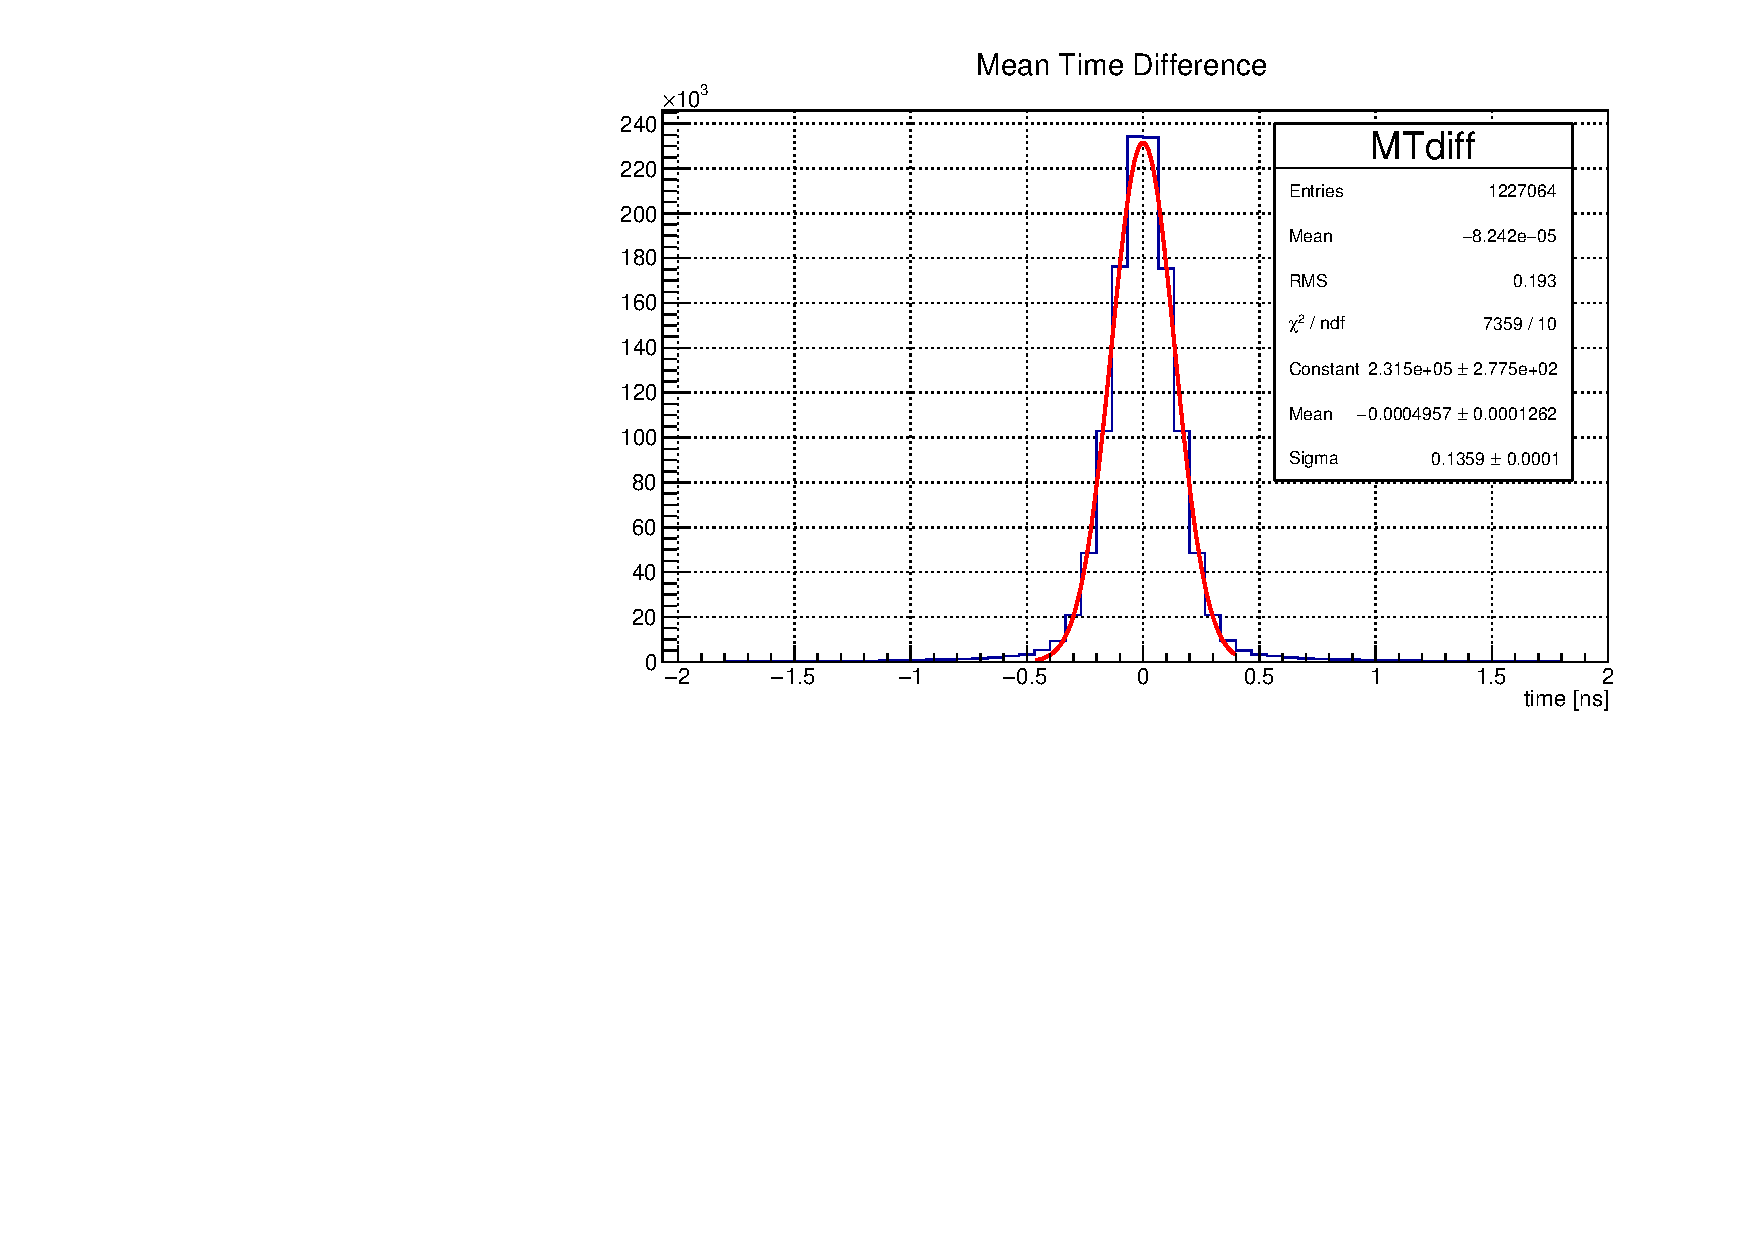
\includegraphics[width=0.8\textwidth]{figures/mt_diff_fullTOF.pdf}
\caption{\label{fig:mt_diff} Mean time difference between one long paddle of one plane with all other long paddles
of the other plane. (Color online)}
\end{center}
\end{figure}
\subsection{Performance \label{sec:scperformance}}
To investigate the performance of the TOF detector for its PID capability it is important to include the relative number of
particle types within the event sample. Here events are selected that do have at least three fully reconstructed charged tracks in the final state with at least one of these tracks intersecting with the TOF detector. The number of pions in such samples will
be much larger than for kaons. The number of protons will be certainly larger than kaons since the data is taken with a hydrogen 
target. Looking at the distribution of $beta$ of these tracks as a function of momentum it is easy to identify the bands
from protons, kaons and pions (see Fig.~\ref{fig:betavsp}). 

Looking at $\beta$ at two specific track momenta of 2~GeV/c and 4~GeV/c, respectively (see Fig.~\ref{fig:betaproj}) is very illustrative to see the limitations
of the TOF detector in terms of PID. At 2~GeV/c particle momentum the TOF detector provides about a 4$\sigma$ separation between
the pion,lepton peak and the kaon peak. This is sufficient to identify tracks with a $\beta$ of 0.97 or lower as kaons with a very
high certainty. However, at a $\beta$ of 0.98 the probability of the track begin a kaon is less than 50\% mainly due to the fact
that the abundance of pions is close to an order of magnitude larger than kaons. The protons on the other hand are very well
separated from the other particle types and can be identified as such with high confidence over the full range in $\beta$.
At a track momentum of 4~GeV/c this has changed and represents the limit at which the TOF can identify protons with high confidence. Again the separation between the large peak containing now pions, kaons and leptons is separated from the proton
peak by about 4$\sigma$, while the relative abundance in this case is about a factor of 4. As a consequence a 4~GeV/c momentum
track with a $\beta$ of 0.975 is most likely a proton with a small probability of being a pion. At a $\beta$ of 0.98 such
a track has a similar probability for being a proton or a pion.
\begin{figure}[tbp]
\begin{center}
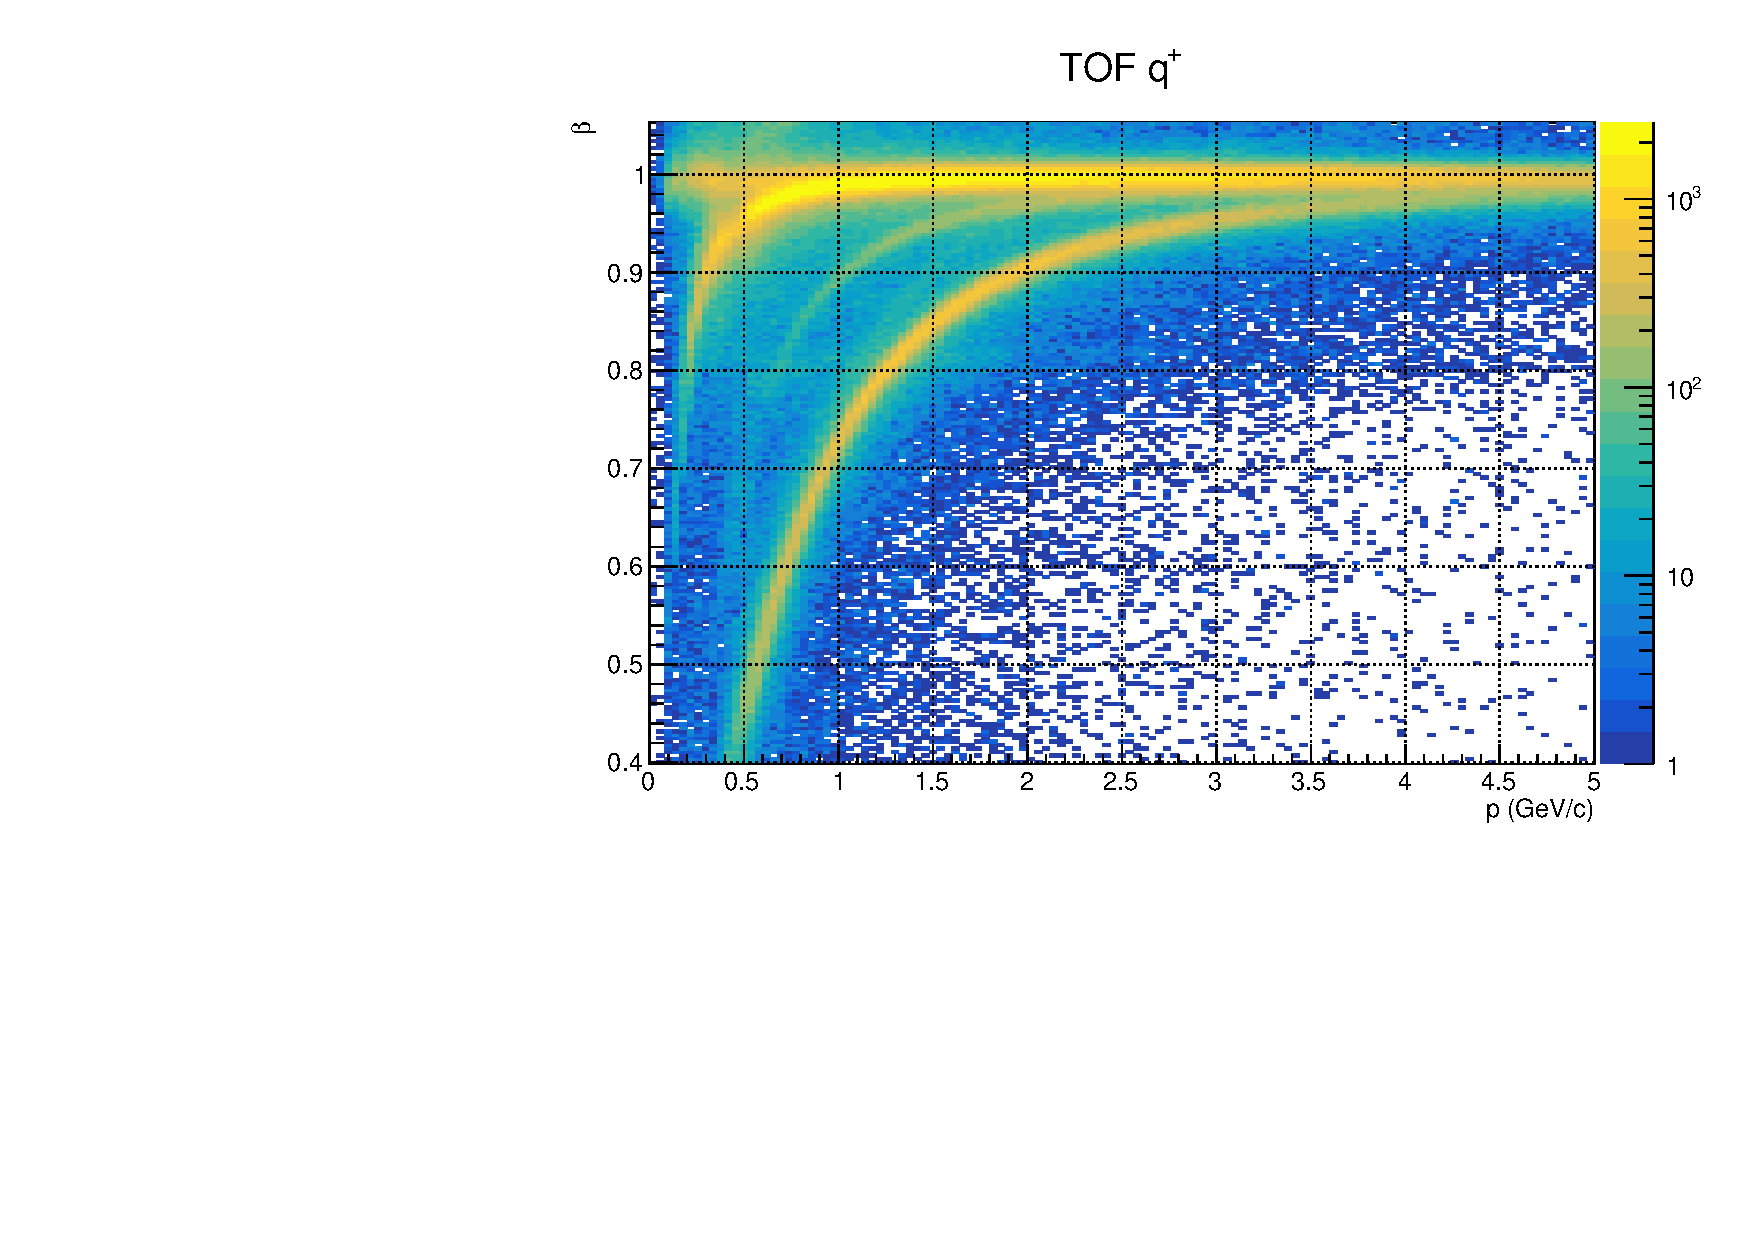
\includegraphics[width=0.8\textwidth]{figures/beta_vs_p_positivetracks.pdf}
\caption{\label{fig:betavsp}$\beta$ of positive charged track vs track momentum. The color coding of the third dimension
is in logarithmic scale.(Color online)}
\end{center}
\end{figure}

\begin{figure}[tbp]
\begin{center}
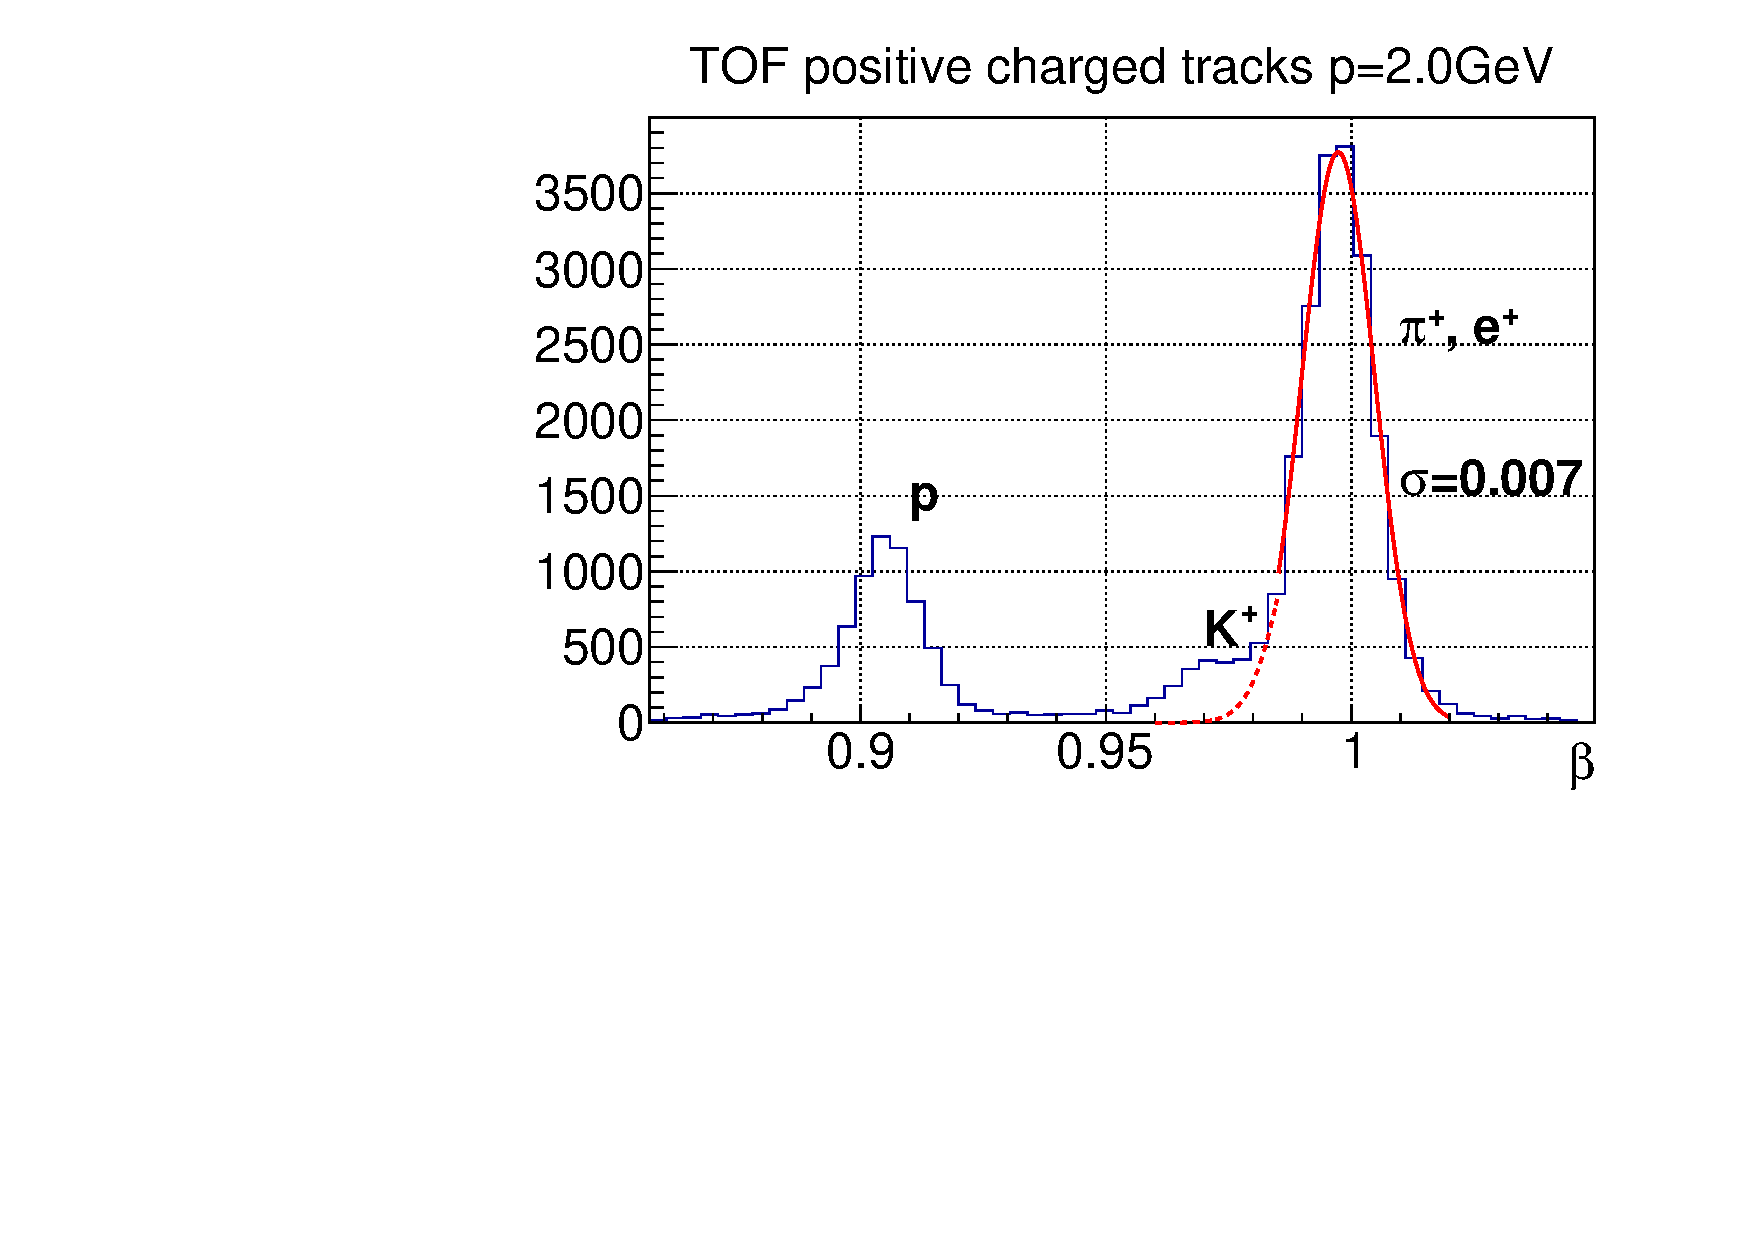
\includegraphics[width=0.45\textwidth]{figures/TOF_postracks_2000mev.pdf}
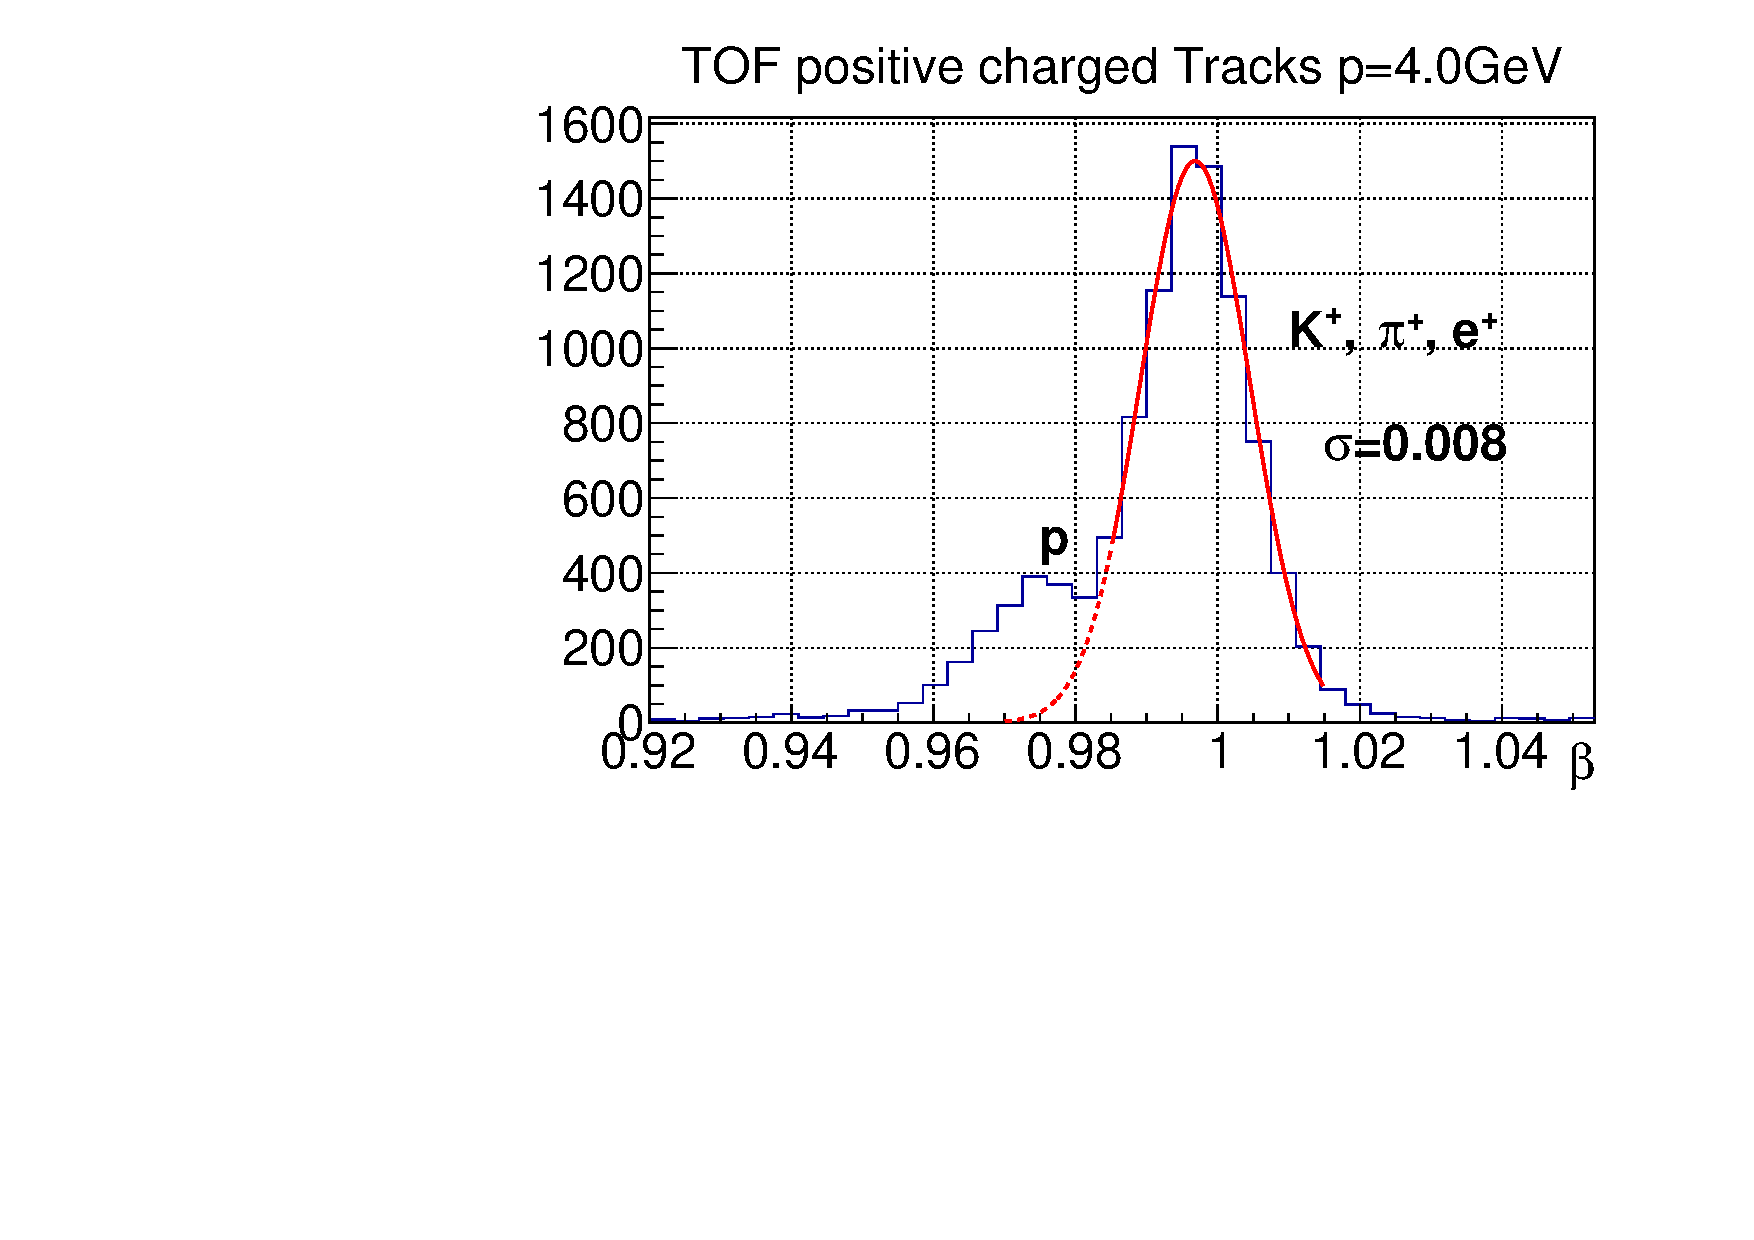
\includegraphics[width=0.45\textwidth]{figures/TOF_postracks_4000mev.pdf}
\caption{\label{fig:betaproj}$\beta$ of positive charged track with 2~GeV/c momentum (left) and with 4~GeV/c (right).}
\end{center}
\end{figure}

\subsection{Summary \label{sec:scsummary}}
The TOF detector in the forward region of the GlueX spectrometer provides high resolution timing information that contributes
to the identification of the RF beam bucket of the beam photon that initiated the event. In combination with the charged
track reconstruction TOF hits can be matched to such tracks to determine $\beta$ and as such give access to the particle
mass of the track. Protons can be identified with reasonable confidence up to momenta of 4~GeV/c while kaons can be
identified up to momenta of 2~GeV/c.
